\documentclass[11pt,norsk,a4paper]{article}
\usepackage[utf8]{inputenc}
\usepackage{babel,csquotes}
\usepackage[T1]{fontenc}
\usepackage[pdftex]{graphicx}
\usepackage{relsize}
\usepackage[hyphens]{url}

% illustrasjonene er laget i powerpoint i filen illustrasjoner.ppt
% og kan revideres der.

% her kommer biblatex-tingene
% sjekk evt for definisjoner
% /local/store/localhost/.texmf-ctan-biblatex/ver-2.4/opt/texlive/texmf-local/tex/latex/biblatex  
\usepackage[%
backend=biber,%
style=numeric,%
sorting=none,%
hyperref=true,%
backref,%
date=long,%
urldate=short,%
]{biblatex}
\addbibresource{referanser.bib}

% lokale biblatex tilpasninger
\DefineBibliographyStrings{norsk}{%
urlseen={Sett: },
%bibliography = {Bibliografi},
%references = {Referanser},
%editor = {redaktør},
%translator={oversetter},
%page={side},
%pages={sidene},
and={og},
}

\DeclareFieldFormat{url}{\url{#1}} % fjerner hardkodet "URL: " foran url
\DeclareUrlCommand\url{\def\UrlLeft{\newline}\def\UrlRight{\newline}%
\urlstyle{sf}} % setter inn passende linjeskift

% biblatex anbefaler at hyperref-pakken lastes inn etter biblatex
\usepackage[colorlinks, allcolors=blue]{hyperref}

% her er mine spesialkommandoer
\newcommand{\kdo}[1]{\texttt{#1}}
%\newcommand{\pil}{$>\ $}
\newcommand{\pil}{ > }
\newcommand{\prikk}{$\bullet\ $}
\newcommand{\en}{EndNote{}}
\newcommand{\bt}{BibTeX{}}
\newcommand{\blt}{B{\smaller[2]IB}\discretionary{-}{}{\kern
    -0.12em}\LaTeX{}}
\newcommand{\underskrift}[1]{\vspace{.2cm}\noindent\textbf{#1}\newline}
\newcommand{\flipp}{\vspace{0.1cm}\newline\indent}
\newcommand{\mnd}{Obligatorisk}
\title{\blt -- kursnotater}
\author{Informatikkbiblioteket\\Universitetet i Oslo}
%\date{22. og 23.januar 2014}

\begin{document}

\maketitle{}
\begin{center}
 {\footnotesize Farget tekst er lenker.}
\end{center}

\tableofcontents
\newpage
\section*{Forord}
Dette notatet er for det meste anvisninger for utførelse av praktiske
øvelser med referanser i \blt. Det er skrevet for å lette
gjennomgangen av øvelsene og for å minske behovet for å gjøre notater
underveis.

Det er i stor grad bygget på oppbygging av 
referanselista til artikkelen om \textit{User interface} i
Encyclopedia of computer science\cite{jacob00-2}.

% \section{Bibliografier og referanselister}

% Dette avsnittet er skrevet som en generell orientering og kan hoppes
% over av dem som vil komme fort i gang.

% \subsection*{Hva er en bibliografi?}
% Bibliografier er litteraturfortegnelser som er ment å dekke et område mer
% eller mindre fullstendig. 

% Det fins f.eks bibliografier som er ment å dekke et fagfelt ved å gi
% oversikt over (all) litteraturen som er publisert innen dette
% fagfeltet.
% \begin{itemize}
% \item Innenfor informatikkfeltet fins det fagbibliografier for spesialfelt
% samlet på et nettsted. \textit{The Collection of Computer Science
%   Bibliographies}\cite{achilles} har bibliografier for en rekke
% informatikk-kategorier som f.eks.

% \textit{Artificial Intelligence; Compiler Technology, Programming Languages
%  and Type Theory; Database Research; Computer Graphics and Vision;
%  Parallel Processing;  Software Engineering and Formal Methods; med flere.}

% \noindent Til sammen over 3~000~000 referanser. I denne tjenesten kan
% man hente referanser ferdig formatert for \bt, men ofte med noe
% ``rufsete'' data, ikke kopiér ukritisk..

% \item\textit{Digital Bibliography \& Library Project} (DBLP - se vår
% hjemmeside) har for det meste tidsskriftartikler og konferanseinnlegg
% og leverer referanser formatert i \bt.

% \item\textit{Nasjonalbibliografier} er en annen type bibliografi. De dekker
% alt som utgis innen et land (f.eks Norsk bokfortegnelse) og produseres
%  vanligvis av nasjonalbibliotekene.

% \item{}Det fins også \textit{personbibliografier}, f.eks. fins det en
%   bibliografi over Arne Næss' skrifter.
% \end{itemize}

\subsection*{Hvorfor referere, hva er en referanseliste?}
Ingen masteroppgave kan leveres uten en referanseliste. Det vil si en
liste over hvilke andre vitenskaplige resultater man bygger på
og/eller viderefører. Hva referanselista inneholder 
og hvordan den ser ut er en viktig faktor i bedømmelsen
av oppgaven. Den viser at forfatteren har oversikt og kjenner til
forskningen på feltet som omtales og at han ikke forsøker å gi
inntrykk av at resultater er hans egne som egentlig tilhører en annen
(plagiat).

Derfor må viktige resultater som oppgaven bygger på, dokumenteres,
eller refereres. Dersom man tar tekster fra et annet dokument, må
dette også tydeliggjøres både ved typografiske virkemidler (eget
avsnitt, anførselstegn, kursiv) og ved referanser til kilden. Viss det
ikke gjøres, blir det å betrakte som plagiering og fusk. Dette har med
intellektuell redelighet å gjøre.

Dersom du gjengir en definisjon av et begrep, er det også viktig å
vise til kilde. Referanser kan også brukes for å knytte seg til en
faglig ``skole'' eller miljø. Alle skrifter som nevnes og/eller brukes
i oppgaven skal være med i referanselista.

Men hvor langt skal man gå i å referere? Skal hver påstand belegges med
referanse til når og av hvem den først ble framsatt? Her er praksis
forskjellig fra fag til fag. Noen belegger nesten alt, til og med det
som må betraktes som allmenne sannheter som at planetene beveger seg i
en bane rundt sola\cite{copernicus}.

Andre nøyer seg med å referere til det som angår oppgavens
problemstilling og -behandling. Det som er allment kjent i fagmiljøet
er det ikke nødvendig å referere. Det går ikke an å gi noen nøyaktige
anvisninger, så det kan være en idé å diskutere nivået med veileder.

Når man refererer, er det et poeng å referere til primærkilden og ikke
andres gjengivelse av primærkilden. Det er ikke sikkert at
sekundærkilden har forstått og gjengitt primærkilden korrekt. Forsikre
deg om at du selv har forstått kilden og gjengir den korrekt.



\subsection*{Viktigheten av korrekte og detaljerte referanser.}
Hensikten med referanselista er at forskningsarbeidet
ditt skal kunne bedømmes korrekt. Da må man gi den som skal bedømme
rimelige vilkår ved å gi nok  detaljerte og korrekte opplysninger
til at kilden eller det refererte materialet er enkelt å finne
tilbake til.

Dette kurset handler om å lage en akseptabel referanseliste ved hjelp
av verktøyet \blt.

\section{Bib-fil og Emacs}
\subsection{Dokumentasjon}
Det anbefales å lese den lokale \blt-guiden\cite{langmyhr13}. Den
inneholder det meste av det du trenger å vite for praktisk
bruk. Ønsker du å dykke ned i materien, fins det en manual\cite{biblatex}.

% Biblioteket er i ferd med å lage en \textit{Guide til \blt} i
% bloggform. Her er det mulig å stille spørsmål og komme med egne
% kommentarer til informasjon biblioteket legger ut. Adressen er:
% \url{http://bibtexuio.wordpress.com/}.

Det fins en wiki-bok om \LaTeX\ som inneholder mange nyttige veiledninger
og tips om bibliografihåndtering med \bt. Den har også en kortere 
beskrivelse av \blt\cite{wikibook}.

%\subsection{GUI for BibTeX}
%Det fins verktøy for å håndtere BibTeX-referanser. 
%\begin{itemize}
%\item\textit{JabRef} og kan lastes ned fra
%\url{http://jabref.sourceforge.net/}. Det er skrevet i Java og skal gå
%på plattformer som Windows, Mac og Linux.
%\item\textit{Zotero} er et elegant tillegg (add-on) til Firefox. Du
%  kan laste det ned fra \url{http://www.zotero.org}. Programtillegget
%  kan brukes for å samle og redigere referanser fra nettsider og
%  deretter eksportere dataene til en bib-fil som kan brukes med
%  \LaTeX.
%
%Zotero ble også omtalt på masterintroduksjonen, som du finner
%via\newline
%\url{http://tinyurl.com/ifibib}
%\end{itemize}

\subsection{bib-filen}
Referansene samles opp i en eller flere filer med filtypen
\textit{bib}. Forbindelsen mellom siteringene i brødteksten
(\LaTeX-filen) og referansene i bib-filen utføres ved bruk av
identifikatorer (mer om dette nedenfor).

\blt-filen kan ligge i samme filkatalog som \LaTeX-filen, men om du
legger den i \verb=~/texmf/bibtex/bib=-katalogen, så vil \blt\ uansett
finne den.


\subsection{Emacs}
Lag en mappe (filkatalog) med navn \textit{biblatexkurs} på ditt
hjemmeområde og lokalisér deg til denne mappen. I Linux ser det slik ut:

\verb=       > mkdir biblatexkurs =

\verb=       > cd biblatexkurs =

\noindent{}Åpne en fil med navnet \textit{minereferanser.bib} i Emacs med denne
kommandoen (Linux):

\verb=       > emacs minereferanser.bib &=

\noindent{}Emacs tar i bruk en egen \bt-modus når du åpner en fil med filtype
\textit{.bib}.  Du får en egen toppmeny i Emacs som heter \textit{Entry-Types}. Når du
skal legge inn en ny referanse, velger du referansetype fra denne
menyen. Fra og med versjon 24.2 kan du i denne menyen velge hvilken \bt-dialekt du vil bruke. Utvalget av dokumenttyper og -felt er forvalgt til å gjelde \bt, men kan stilles om til å gjelde \blt\ ved valget nederst i \textit{Entry-types}-menyen. Velg \blt.

Når du har valgt referansetype, får du opp en referansepost med bare
tomme felter, f.eks. slik (\textit{article in journal} eller Ctrl-c Ctrl-e
Ctrl-a):

{\footnotesize\begin{verbatim}
    @Article{,
      author =       {},
      title =        {},
      journaltitle = {},
      ALTyear =      {},
      ALTdate =      {},
      OPTvolume =    {},
      OPTnumber =    {},
      OPTpages =     {},
      OPTmonth =     {},
      ...
    }
\end{verbatim}}




\subsection*{Identifikatorer}
Referanser i \blt\ må ha en identifikator som er entydig. Den skal
ligge rett etter første krøllparentes og avsluttes med komma. Den
brukes når du seinere skal sitere referansen.

En slik identifikator bør være enkel å huske. Eksempler på identifikatorer: \textit{shneiderman1983},
\textit{olsen1992}.  

\subsection*{Felter}
De feltene som innledes
med \textit{OPT} er valgfrie, resten er obligatoriske. Av og til kan
to eller flere felt innledes med \textit{ALT}. Da må man fylle ut ett
av dem. Velg \textit{Book} fra Entry-menyen for et eksempel.

Teksten i feltene må enten være omsluttet av krøllparenteser
(\verb={}=) eller doble anførsel (\verb=" "=). Unntakene fra
denne regelen er året (year) som kan angis med fire siffer, andre rene tall og
makroer (se avsnitt~\ref{makroer}).

Feltene skal skilles av komma.

\subsection*{Forfatterfeltet}
Forfatter-feltet heter \textbf{author}. Her oppgis navn, enten rett
fram eller med etternavn etterfulgt av komma. \blt\ forsøker å splitte
et rett fram-navn i fire deler: fornavn, mellomnavn av typen \textit{von, van,
  de, \ldots}, så etternavn og til slutt navnetillegg av typen
\textit{junior, senior, \ldots}. Forsøket lykkes ikke alltid, så det
sikreste er å oppgi etternavn etterfulgt av komma etterfulgt av resten
av navnet.

Flere forfattere skilles av teksten
\textbf{and}.

Initialer i personnavn skal registreres med punktum og mellomrom,
slik: \texttt{Knuth, D. E.}.

Tilsvarende gjelder for andre felt som inneholder ett eller flere
personnavn: \textbf{editor, translator,\ldots}.

Generelt bør navn registreres fullt ut (uten initialer). Da kan man la
stilen bestemme hvorvidt det skal skrives med initialer eller fullt navn.

Kjenner du ikke fullt navn, så sørg likevel for at du gir samme forfatter ens navn.

\subsection*{Store bokstaver }
Opplysningene i noen felt kan bli redigert av \bt\ dersom dokumentstilen krever
det. F.eks. kan store bokstaver bli omgjort til små. Det skjer ikke i \blt. For å omgå dette,
kan man sette teksten man ønsker å beholde i krøllparenteser. Særlig
aktuelt er dette i forbindelse med forkortelser (``ACM'', ``IEEE'') og
egennavn som forekommer i f.eks. tittel. 


\subsection{Makroer\label{makroer}}
Enkelte opplysninger opptrer ofte. Det kan være navn på tidsskrifter,
forlagsnavn og person- og institusjonsnavn. For å spare tastearbeid og
å sikre konsistens kan man for slike tilfeller bruke
\textit{makroer} eller \textit{aliaser}. Disse defineres i begynnelsen av
bib-filen. Eksempler:

{\footnotesize
\begin{verbatim}
  @string{ben   = "Shneiderman, Ben"}
  @string{ojd   = "Dahl, Ole-Johan"}
  @string{tochi = "ACM Transactions on Computer-Human Interaction"}
  @string{aw    = "Addison-Wesley"}
\end{verbatim}
}

\noindent{}Man kan ikke kombinere forfattermakroer i samme author-felt. 
Man kan i stedet lage en egen makro for kombinasjonen av forfattere\footnote{Se eksempel 
i tex-filen vi bruker seinere i kurset.}. Makroer vil bli ekspandert i løpet av prosesseringen. 
Har man definert ovennevnte makroer, kan man skrive (uten anførsel eller krøllparenteser):
{\footnotesize\begin{verbatim}
    author = ojd,
    editor = ben,
    journaltitle = tochi,
    publisher = aw,
\end{verbatim}}

\subsection{De viktigste referansetypene}\label{bibtextyper}

Her omtales bare de viktigste referansetypene. For hver type oppgis
obligatoriske og anbefalte felt. I de fleste tilfellene vil programmet \textbf{biber} foreta
konvertering av felt fra \bt{} til \blt. Biber er programmet som
genererer referanselista\footnote{Databasene vi skal hente referanser
  fra leverer \bt-referanser, ikke \blt.}.

\underskrift{Article -- artikkel i tidsskrift}
\indent\begin{tabular}{ll}
\mnd:&\textit{author, title, journaltitle, year/date}\\
%\bt: &\textit{author, title, journal, year}\\
Anbefalt:& \textit{volume, number, pages}.\\ 
\end{tabular}

\underskrift{Book -- bok}
\indent\begin{tabular}{ll}
\mnd:&\textit{author, title, year/date}\\
Ved behov: &\textit{edition}\\
%\bt: &\textit{title, publisher, year} og én av\\
%&\textit{author} eller \textit{editor} (redaktør).\\ 
\end{tabular}

\underskrift{InBook -- del av  bok}
\noindent{}Typen gjelder en selvstendig del av en bok med egen tittel.
\flipp\begin{tabular}{ll}
\mnd:&\textit{author, title, booktitle, year/date}.\\
%\bt: &\textit{author/editor, title, chapter, publisher, year}.\\
Anbefalt: &\textit{publisher, pages}.\\
\end{tabular}

\underskrift{Collection -- samling/antologi}
\indent\begin{tabular}{ll}
\mnd:&\textit{editor, title, year/date}\\
Anbefalt:&\textit{publisher}\\ 
\end{tabular}

\underskrift{InCollection -- kapittel i bok}
\noindent{}Typen er beregnet på selvstendige bidrag i en samling. Bidraget har egen forfatter og tittel. \texttt{author} og \texttt{title} henger sammen og analogt: \texttt{editor} og \texttt{booktitle}.\flipp\begin{tabular}{ll}
\mnd&\textit{author, editor, title, booktitle, year/date}. \\
%\bt &\textit{author, title, booktitle}. \\
Anbefalt: &\textit{publisher, year}.\\ 
\end{tabular}

\underskrift{Proceedings -- konferanserapport}
\indent\begin{tabular}{ll}
\mnd:&\textit{title, year/date}. \\
%\bt: &\textit{title, year}. \\
Anbefalt: &\textit{editor, publisher}.\\ 
\end{tabular}

\underskrift{InProceedings -- konferanseinnlegg}
Denne er analog med \verb=@incollection=.
\flipp\begin{tabular}{ll}
\mnd:&\textit{author, title, booktitle}. \\
%\bt: &\textit{author, title}. \\
Anbefalt: &\textit{year, publisher, pages}.\\ 
\end{tabular}

\underskrift{Thesis -- avhandlinger (master, doktor)}
Avhandlingstype angis i type-feltet (master, phd).
\flipp\begin{tabular}{ll}
\mnd:&\textit{author, title, type, institution,
  year/date}. \\ 
%\bt: &\textit{author, title, school, year}. \\ 
\end{tabular}

\underskrift{Report -- teknisk rapport}
Rapporttype må oppgis ved avvik fra forvalgt verdi (''technical
report'').
\flipp\begin{tabular}{ll}
\mnd:&\textit{author, title, type, institution, year/date}\\
%\bt: &\textit{author, title, institution, year}\\
Anbefalt: & \textit{number}(rapportnummer)\\ 
\end{tabular}

\subsection{Kryssreferanser: crossref-feltet} 
Dersom man skal registrere flere bidrag fra samme bok, samling eller
konferanse, er det tungvint å registrere boktittel/konferansenavn og
andre fellesopplysninger flere ganger.

Man kan f.eks i \textit{inBook}-posten angi et crossref-felt som
inneholder identifikatoren til relevant \textit{Book}-post. Se
figur~\ref{crossref}. Tilsvarende gjelder for
\textit{inProceedings/proceedings} og
\textit{inCollection/collection}.

\begin{figure}
\begin{center}
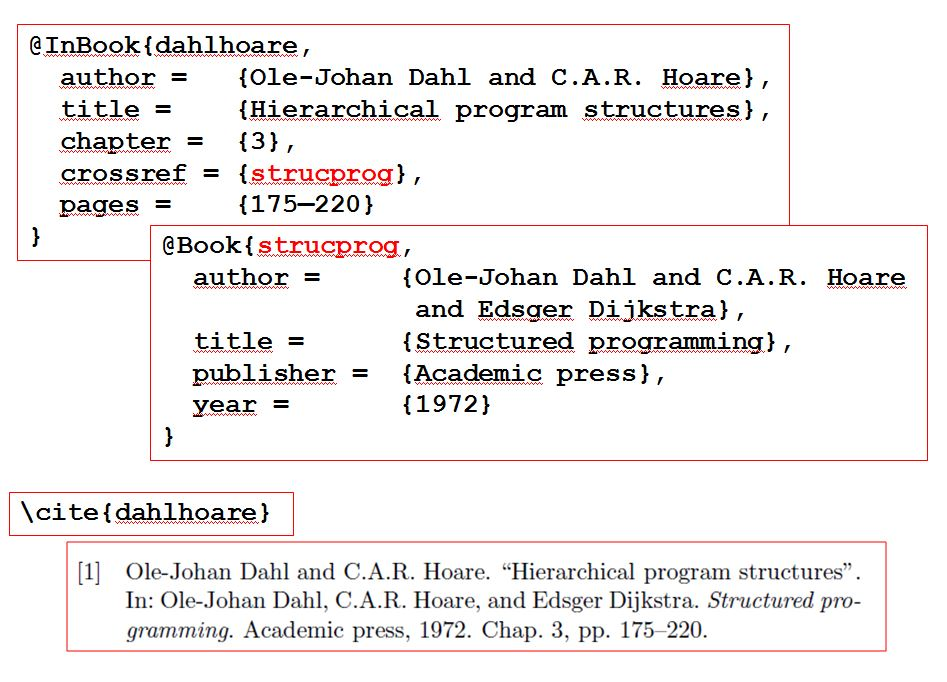
\includegraphics[width=10cm]{./chapterinbook.jpg}
\caption{Bruk av referansetypene inBook og Book med
  kryssreferanse.}\label{crossref}
\end{center}
\end{figure}

\subsection{URL-er}\label{biblatex-url}
Alle referansetyper i \blt\ kan ha feltet \textit{url}. Når dette
brukes, bør man også bruke feltet \textit{urldate} for å vise når
url-en sist ble aksessert. Dette er viktig av flere grunner:
web-sider endrer seg over tid og du må si hvilken versjon du refererer
til. Dessuten skifter dokumenter ofte URL i tidens løp.
Datoen vil bli satt i parentes med ``sjekket'' eller ``visited on''
som prefiks om man ikke gjør noe annet. Prefikset er innholdet av
variabelen \texttt{urlseen}, som kan redefineres om du ønsker en annen
tekst, se avsnitt~\ref{tekster} på side~\pageref{tekster}.

Det anbefales at du skriver ut en kopi av nettsiden for eventuell
seinere kontroll. 

% URL-en vil i \blt\ bli prefikset med ``URL:'' som default. Denne teksten kan
% endres ved følgende kommando i innledningen, slik:

% \begin{verbatim}
%      \DeclareFieldFormat{url}{dinegentekst\url{#1}} 
% \end{verbatim}



\subsection{Datoformat}
Datoformatet avhenger av dokumentspråk og format. Sier man ikke noe, gir
\textbf{norsk} 29.07.2013, og \textbf{english}  07/29/2013. Man kan
også stille inn datoformatet som pakkevalg og man kan da skille mellom
vanlig \textbf{date} og \textbf{urldate} og andre datoer, se nærmere
om valgmuligheter i \cite[][50--53]{biblatex}.

\section{Øvelse 1: Samle referanser i en bib-fil} Vi skal nå fylle opp
bib-filen med referanser. Dels ved å hente ferdig formaterte
referanser fra ulike kilder, dels ved å skrive inn. Referansene fins
på et eget ark som også er referanselista til dette dokumentet.
Bibliografien til leksikon-artikkelen inneholder 11 referanser
\cite{hutchins1986,olsen1992,johnson1989,shneiderman1983,hartson1989,jacob1986,myers1995,foley1990,foley1987,shneiderman1992,stephenson1999}. Vi
skal behandle noen eksempler i detalj og deretter kopiere en ferdig
bib-fil fra nett.

Vanligvis vil du laste ned referansen samtidig med at du laster ned
dokumentet. Gjør du det til en vane, så sparer du deg selv for mye
arbeid seinere.

\begin{itemize}

\item\textbf{Hutchins et al., 1986 \cite{hutchins1986}}\newline Vi går
  til \textit{Google Scholar} via bibliotekets hjemmeside (\href{https://www.ub.uio.no/informatikk}{lenke}). Klikk på
  \textit{Innstillinger} i horisontalmenyen. Under avsnittet
  \textit{Bibliography Manager} krysser du av for \textit{Show links
    to import citations into} og velger \textit{BibTeX} i
  menyen. Lagre innstillingene ved å klikke på \textit{Save
    preferences}.

  Finn fram referansen ved å søke på de tre forfatternavnene
  \textbf{Hutchins Hollan Norman} og klikk på \textit{Import into BibTeX}
  ved første treff. Referansen dukker da opp i BibTeX-syntaks. Er det
  riktig referanse?\footnote{Nei. Hvorfor ikke?} Kikk på mulige
  referanser lenger ned på sida. Reagerer du på noe
  spesielt?\footnote{Veldig upresise referanser og mange basert på
    siteringer.} Heller ikke de 26 versjonene bringer oss til målet, alle er fra 1985.

  Vi prøver den samme referansen (\cite{hutchins1986}) i
  \textbf{Collection of Computer Science Bibliographies}\cite{achilles}.

Klikk på \textit{Search} og skriv deretter inn hutchins, velg author
som søkefelt og 1986 som år.

Tredje treff er den vi er på jakt etter. Klikk først på ``5
duplicates'' og se samme dokument presentert på forskjellig måte
(forskjellige kilder). Studér forskjellene. Gå tilbake til trefflista
og klikk så på \bt-lenken til høyre
for referansen. Kopier \bt-referansen fra nettleseren og inn i
bib-filen.

\item\textbf{Olsen, 1992 \cite{olsen1992}}\newline Vi gir Google
  Scholar en ny sjanse med \cite{olsen1992}.  Søk på \textit{olsen
    user interface management}. I skrivende stund øverst i trefflista.

Klikk på lenken \textit{Import into \bt}. Er den OK?\footnote{Ja.}

\item\textbf{Din egen masteroppgave}\newline Velg riktig entry-type fra
  menyen og fyll inn de obligatoriske feltene. Gi kommandoen
  \kdo{Ctrl-c Ctrl-c} for å rydde opp og generere identifikator.

\item\textbf{Johnson et al., 1989 \cite{johnson1989}}\newline 
Gå til IEEE Xplore via bibliotekets hjemmeside og søk på \textit{johnson
xerox star}. 

Merk av referansen og trekk ned menyen \textit{Download citations}
over trefflista. Velg \textit{BibTeX} og \textit{Citation only} og
klikk på \textit{Download}. Kopier referansen inn i
bib-filen.

% \item\textbf{Shneiderman 1983 \cite{shneiderman1983}}\newline 
% Du finner også denne referansen i \textbf{IEEE Xplore}. Søk på
% \textit{shneiderman 1983} og følg prosedyren
% fra forrige punkt.

\item\textbf{Hartson, 1989\cite{hartson1989}}\newline
Denne referansen vil du finne i \textit{ACM Digital Library}.

  Generell beskrivelse av framgangsmåten: I en treffliste klikker du
  på aktuell tittel. Da vil du komme til en side som har en grå boks i
  høyremargen -- \textit{Tools and Resources}. Nederst i boksen finner
  du lenken \textit{\bt}. Bruker du den, får du opp
  referansen i et eget vindu og kan klippe og lime den inn i din egen
  bib-fil.

  Gå til ACM Portal via bibliotekets hjemmeside. Velg ACM Digital
  library og klikk på journals (under overskriften \textit{Browse the
    digital library} og finn fram \textit{Computing
    surveys}\footnote{Bruk evt Ctrl-F for å søke på siden.}, gå til
  arkivet og finn fram riktig volum (21 -- 1989). Klikk på riktig
  nummer (1) og deretter på innholdsfortegnelsen-fanen (Table of
  contents).

Finn fram referansen og se på den. Legg merke til at ACM forkorter
tidsskriftnavnet.  Dette kan du rette opp når du har kopiert
referansen over til bib-filen.

% \item\textbf{Jacob, 1986 \cite{jacob1986}}\newline Bruk \textit{ACM
%     Digital Library}. Se forrige punkt. Rett opp tidsskriftnavnet.

% \item\textbf{Myers, 1995 \cite{myers1995}}\newline Use \textit{ACM
%     Digital Library}. Se forrige punkt. Bytt ut tidsskriftnavnet
%   (journal-feltet) med den makroen du laget i starten
%   (\texttt{atch}). Husk: ingen krøllparenteser her.

% \item\textbf{Foley, 1990 \cite{foley1990}}\newline Bruk
%   \textit{Collection of Computer Science Bibliographies} (CCSB). Klikk
%   på \textbf{Search} i horisontalmenyen. Skriv \textit{Foley} i
%   søkefeltet, velg \textit{author} som kvalifikator og \textit{1990}
%   som publikasjonsår.

% \item\textbf{Foley, 1987 \cite{foley1987}}\newline
% Bruk \textit{Collection of
%   Computer Science Bibliographies} (CCSB). Se forrige punkt.

% \item\textbf{Shneiderman, 1992 \cite{shneiderman1992}}\newline
% Bruk \textit{Collection of
%   Computer Science Bibliographies} (CCSB). Se ovenfor.

% \item\textbf{Stephenson, 1999 \cite{stephenson1999}}\newline
% Bruk \textit{Collection of
%   Computer Science Bibliographies} (CCSB). Se ovenfor.
\end{itemize}

Resten av referansene i lista følger disse rutinene. Som en øvelse kan
du etter kurset finne og hente referansene på egen hånd\footnote{Du finner 
\cite{shneiderman1983} i IEEE Xplore,
\cite{jacob1986,myers1995} i ACM Digital library og 
\cite{foley1990,foley1987,shneiderman1992,stephenson1999} i Collection of Computer Science Bibliographies.}. Vi bruker ikke tid på dem, men laster ned en bib-fil fra :

{\footnotesize\begin{verbatim}
        http://folk.uio.no/knuthe/biblatex/nor/
\end{verbatim}}
\noindent{}Høyreklikk på \textbf{referanser.bib} og last ned.

Kopiér inn referansen til din egen oppgave fra den
andre bib-filen.


\section{Øvelse 2: Bruke bib-filen med et dokument}

Grovstrukturen i et \LaTeX-dokument som bruker \blt\ er vist i
figur~\ref{document}. 

I denne øvelsen skal du kopiere teksten fra

{\footnotesize\begin{verbatim}
        http://folk.uio.no/knuthe/biblatex/nor/
\end{verbatim}}
\noindent{}Høyreklikk på \textbf{userinterface.tex} og last ned.

Åpne filen i Emacs. Du skal så arbeide med å sette inn
korrekte siteringer der det er markert med forfatter og årstall mellom
doble stjerner (**).


\begin{figure}
\begin{center}
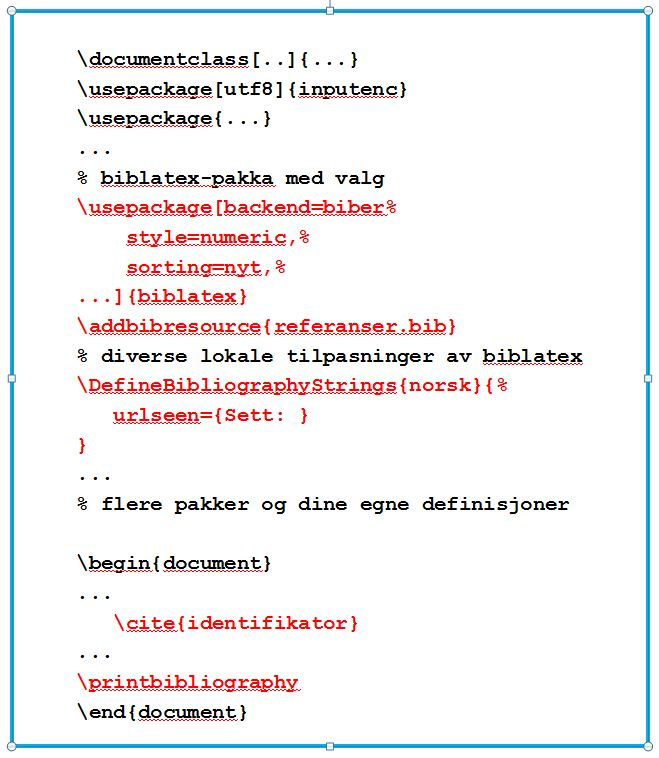
\includegraphics[width=\textwidth]{./documentstructure.jpg}
\caption{Grovskisse av \LaTeX-dokument som bruker \blt (alt i rødt har med \blt å gjøre.}\label{document}
\end{center}
\end{figure}

\subsection{Tegnsett}
I figur~\ref{document} er det skrevet
\verb=\usepackage[utf8]{inputenc}=. UTF8 vil da bli antatt brukt både
i tex- og bib-fil. Dersom man bruker et annet tegnsett i bib-filen må
dette angis som valg til biblatex-pakka:

{\footnotesize\begin{verbatim}
    \usepackage[utf8]{inputenc}
    \usepackage[bibencoding=latin1]{biblatex}
\end{verbatim}}
\noindent{}UTF8 er standard på IFI nå.

\subsection{Én eller flere bib-filer}
Etter å ha lastet inn \blt{}-pakken, må systemet få vite hvilke
bib-filer som skal brukes. Dette gjøres med kommandoen:

{\footnotesize\begin{verbatim}
    \addbibresource{bib-filnavn}
\end{verbatim}}
\noindent{}Bib-filer må oppgis med extension (.bib) og om du bruker flere
bib-filer, må du gi flere kommandoer. Da kan det også være aktuelt å samle
alle makroer i en egen fil. Den må da lastes inn først:

{\footnotesize\begin{verbatim}
    \addbibresource{makroer.bib}
    \addbibresource{library1.bib}
    \addbibresource{library2.bib}
\end{verbatim}}

\subsection{Sitering}
Når du skal sitere i \LaTeX, setter du inn en \texttt{cite}-kommando
med identifikatoren som parameter, slik:

{\footnotesize\begin{verbatim}
   \cite{identifikator}
\end{verbatim}}
\noindent{}Identifikatoren må være skrevet nøyaktig slik den er skrevet
i bib-filen (følsomhet for store og små bokstaver).

Ønsker du å sitere flere samtidig, skilles de av komma innenfor
krøllparentesene: 

{\footnotesize\begin{verbatim}
   \cite{identifikator1,identifikator2}
\end{verbatim}}
\noindent{}Du kan oppgi tekst som skal inngå foran eller bak selve
siteringen.

{\footnotesize\begin{verbatim}
   \cite[prefiks][suffiks]{identifikator}
\end{verbatim}}
\noindent{}Om man ønsker å vise til en bestemt side i det dokumentet
man siterer, så kan det ordnes med klamme-parametre til
cite-kommandoen:

{\footnotesize\begin{verbatim}
   \cite[Se også][47]{identifikator}
\end{verbatim}}
\noindent{}som vil komme ut som: \verb=[Se også 19, s. 47]=. Se \cite[][14]{langmyhr13} for flere \verb=\cite=-kommandoer.

Om du ikke direkte siterer en referanse du har i bib-filen,
men ønsker å ha den med i referanselista, kan du skrive:

{\footnotesize\begin{verbatim}
   \nocite{identifikator}
\end{verbatim}}
\noindent{}Du kan her bytte ut \textit{identifikator} med *. Da kommer alle
referansene i bib-filene med i referanselista.

\subsection{RefTeX -- finne fram og velge referanse}
\subsubsection*{Emacs i RefTeX-modus}
Det fins et tillegg til Emacs -- RefTeX -- som gjør det enklere å
håndtere siteringer\cite{reftex}. Pakken kan anbefales også av andre
grunner, den kan f.eks. hjelpe deg å holde orden på interne
kryssreferanser i \LaTeX-dokumentet.

Før du setter Emacs i RefTeX-modus, må du gjøre en vri. RefTeX er
avhengig av å få vite hvilke bib-filer du bruker. RefTeX er skrevet
for å støtte \bt-logikken og vil hente bib-filen fra en
\kdo{$\backslash$bibliography}-kommando. For å få RefTeX til å fange
opp bib-filer fra \kdo{$\backslash$addbibresource} må følgende legges
inn i din .emacs-fil:

{\footnotesize\begin{verbatim}
(setq reftex-bibliography-commands 
   '("addbibresource" "bibliography" "nobibliography")) 
\end{verbatim}}
Haken er at RefTeX bare fanger opp den første bib-filen angitt med
\textbf{addbibresource}. Bruker du flere bib-filer, må du oppgi dem
samlet i en \textbf{bibliography}-kommando\footnote{Kommandoen må
  ligge i innledningen. Her trengs ikke
  extension .bib}:

{\footnotesize\begin{verbatim}
      \bibliography{makroer, referanser}
\end{verbatim}}

Du kan sette Emacs i RefTeX-modus med kommandoen {\footnotesize \verb=M-x reftex-mode=}.\footnote{M-x betyr først å taste ESC-tasten og deretter bokstaven x} 
Legg merke at du har fått en \textit{Ref}-meny i
toppmenyen.

Du kan også sette Emacs i RefTeX-modus ved oppstart ved å legge følgende
linjer inn i .emacs-filen:

{\footnotesize\begin{verbatim}
   (add-hook 'LaTeX-mode-hook 'turn-on-reftex)
   (autoload 'reftex-mode "reftex" "RefTeX Minor Mode" t)
   (autoload 'turn-on-reftex "reftex" "RefTeX Minor Mode" nil)
\end{verbatim}}

\subsubsection*{Søke i bib-filene}
RefTeX gir deg muligheten til å finne referanser i bib-filen ved å
søke med regulære uttrykk.

Plassér markøren der du vil ha siteringen. Gi kommandoen
\verb=C-c [= eller velg \verb/\cite/-kommandoen fra Ref-menyen,
skriv inn det regulære uttrykket og tast return. Du får da
 en treffliste. Du kan navigere opp og ned i trefflista med
piltastene og velge referanse ved å taste return. Da kommer
cite-kommando med riktig identifikator inn der markøren sto. Dette
gjør det også enklere å operere med identifikatorer som ikke
nødvendigvis er så lette å huske.

Skal du ha flere identifikatorer inn i samme sitering, settes markøren
innafor krøllparentesen. Deretter søker og velger du på ny.

Sett nå inn \verb=\cite=-kommandoer for alle referansene i den
oppgitte teksten.

\subsection{Bibliografiske stiler}
Stiler for siteringer og referanser angis som valg til
\blt-pakken:

{\footnotesize\begin{verbatim}
      \usepackage[...,
       style=stilvalg,
       ...]{biblatex}
\end{verbatim}}

\kdo{style} angir stilvalget for både sitering og referanse samtidig,
men man kan også spesifisere dem hver for seg.

{\footnotesize\begin{verbatim}
      citestyle=stilvalg-1,
      bibstyle=stilvalg-2,
\end{verbatim}}

Her er noen av standardstilene\footnote{Det fins mange flere stiler,
  se \cite[][65-70]{biblatex}.}:

\begin{description}
\item[numeric] -- Siteringen oppgis som et nummer i skarpe
klammer som viser til en nummerert referanseliste. Sorteringen av
referanselista kan styres med et eget valg til \blt-pakka. I 
dokumentet du nå leser er sorteringen \textbf{none} som gir en rekkefølge
bestemt av rekkefølgen av \kdo{cite}-kommandoer.

\item[alphabetic] -- Siteringen er en konstruksjon av
forfatternavn og årstall som settes i
skarpe klammer ($[KNU99]$). Referanselista sorteres ifølge denne konstruksjonen.

\item[authortitle] --  Siteringen blir etternavn og tittel på
verket i kursiv uten parentes rundt. For å få parentes rundt
siteringen må du bruke en annen cite-kommando:
\verb=\parencite=. Referansene i lista får ikke eget merke, men er
sortert etter navn og tittel.

\item[authoryear] -- Siteringen blir etternavn og år for publisering
  uten parentes rundt. For å få parentes rundt siteringen må du bruke
  en annen cite-kommando: \verb=\parencite=. Man kan selvsagt sette
  parenteser rundt \verb=\cite=-kommandoen også. Referansene i lista
  får ikke eget merke, men er sortert etter navn og år.
\end{description} 

Dersom du ønsker å bruke stilen APA (American Psychological Association) eller Chicago, er dette beskrevet i den lokale guiden.\cite{langmyhr13}

\subsection{Generere referanselista}
Der du skal ha inn referanselista i dokumentet, skriver du følgende
kommando:

{\footnotesize\begin{verbatim}
   \printbibliography
\end{verbatim}}
\noindent{}Så gir du følgende kommandoer i terminalvinduet (eller i verktøyet):
{\footnotesize\begin{verbatim}
   > pdflatex userinterface.tex
   > biber userinterface
   > pdflatex userinterface.tex
   > pdflatex userinterface.tex
\end{verbatim}}
\noindent{}Kort fortalt skjer dette: Den første pdflatex-kommandoen genererer en
del mellomlagringsfiler som biber-programmet bruker for å generere
siterings- og referanselisteinformasjon som blir inkludert i
produksjon ved neste pdflatex-kjøring.

Går kjøringene uten feilmeldinger, kan du se resultatet ved å åpne
pdf-filen som er sluttresultatet.

I Linux kommandomodus kan du i IFI-miljø gi kommandoen 
{\footnotesize\begin{verbatim}
   > ltx  userinterface.tex 
\end{verbatim}}
\noindent{}som tar seg av alle de fire skrittene ovenfor.
\subsection{Variere stil}
Når man skal endre stil, kan det være lurt å slette en del
mellomlagringsfiler før ny produksjon 

{\footnotesize\begin{verbatim}
   > rm  *.aux *.bbl *.bcf *.blg *.out 
\end{verbatim}}
\noindent{}Prøv nå å endre stilen til \textit{alphabetic} og kjøre ny produksjon. Sjekk
resultatet.

Så kan du prøve stilen \textit{authortitle}. Legg merke til at du ikke lenger
får parenteser rundt siteringen. Bytt ut \kdo{$\backslash$cite} med
\kdo{$\backslash$parencite} på én av siteringene og sjekk resultatet. Sjekk også sorteringen av
referanselista.

Endre siteringsstilen tilbake til \textit{numeric} og siteringen tilbake til \kdo{$\backslash$cite}.


\subsection{Overskriften til referanselista}
Teksten som skrives ut over referanselista er inneholdt i en
\LaTeX-variabel som brukes som forvalg for \blt{}-variabelen
\kdo{bibliography}.

Dersom dokumentklassen er \textit{article} heter
variabelen \verb=\refname=. Dersom dokumentklassen er \textit{book}
heter variabelen \verb=\bibname=.

Innholdet i variablene avhenger også av
dokumentspråket. I nedenstående tabell~ vises forvalgte verdier for
disse variablene.

\begin{center}
\begin{tabular}{|r|c|c|}\hline
        &\textbf{norsk}&\textbf{english}\\ \hline
\textbf{article}&Referanser&References\\ \hline
\textbf{book}&Bibliografi&Bibliography\\ \hline
\end{tabular}

\end{center}
\noindent{}Dersom du ønsker å endre innholdet i variablene, kan du gi kommandoen

{\footnotesize\begin{verbatim}
   \renewcommand{\refname}{Litteraturliste}
\end{verbatim}}
\noindent{}Overskriften kan også være en parameter til
\kdo{printbibliography}:

{\footnotesize\begin{verbatim}
   \printbibliography[title={Litteraturliste}]
\end{verbatim}}
\noindent{}En tredje variant er nevnt på side~\pageref{heading}.

\subsection{Referanselista i innholdsfortegnelsen}\label{innhold}
Henvisning til referanselista kommer ikke automatisk inn i
innholdsfortegnelsen.  

Rett etter \texttt{printbibliography}-kommandoen kan du skrive kommandoen
\kdo{addcontentsline} i \LaTeX-filen. Viss du setter
innholdet av \verb=\refname= før disse to, så sikrer du konsistens:

{\footnotesize\begin{verbatim}
   \renewcommand{\refname}{Litteraturliste}
   \printbibliography
   \addcontentsline{toc}{section}{\refname}
\end{verbatim}}
\noindent{}Her forteller \textit{toc} at det hele skal inn i table-of-contents,
\textit{section} hvilket dokumentnivå innførselen skal ha og
\verb=\refname= hvilken tekst som skal inn i innholdsfortegnelsen
(her er det innholdet av variabelen \verb=\refname=).


\subsection{Baklengs referering} Når dokumentet er blitt stort, kan
det bli vanskelig å huske hvor man har sitert en spesifikk
referanse. Det fins en mekanisme (i pakken \textit{hyperref}) for å
føye til siterings-sidetall til hver enkelt referanse i
referanselista.

Ved å føye til

{\footnotesize\begin{verbatim}
   \usepackage{hyperref}
\end{verbatim}}
\noindent\textit{etter} \blt-pakken
i innledningen og gi \kdo{backref} som opsjon til \blt{}, så får man ønsket effekt (pluss noen andre, som
interne og eksterne lenker i dokumentet). Pakken \textit{hyperref} er
beskrevet i \cite{hyperref}.

I dokumentet du nå leser, kan du se hvordan det vil se ut i referanselista.

\subsection{Seksjons-, type-, tema- eller kapittelvise referanselister}
\subsubsection*{Referanseliste i hver seksjon}
Du kan generere referanselister for hver seksjon eller kapittel ved å
markere start og slutt på en referanseseksjon. I hver seksjon eller
kapittel brukes \textbf{printbibliography} for å skrive ut inneværende
seksjons referanseliste:

{\footnotesize\begin{verbatim}
   \chapter{...}
      \begin{refsection}
      ...
      \printbibliography
      \end{refsection}

   \chapter{...}
      \begin{refsection}
      ...
      \printbibliography
      \end{refsection}
\end{verbatim}}
\noindent{}Alle siteringer gjort innenfor referanseseksjonen vil inngå i
referanselista. Slik kan man gjøre for alle seksjoner/kapitler.

Eventuelle siteringer gjort utafor en seksjon vil
bli sendt til en slutt-referanse\-liste.

\subsubsection*{Inndelt referanseliste til slutt}

Ønsker du kapittelinndelt referanseliste til slutt i dokumentet,
legger du inn refsection-områder i tex-filen som i forrige avsnitt,
men du skriver ikke ut referanselista i hvert kapittel.

Du kan avslutte dokumentet med følgende kommandosekvens:

{\footnotesize\begin{verbatim}
   \printbibheading
   \printbibliography[section=1, heading=overskrift]
   \printbibliography[section=2, heading=overskrift]
   \printbibliography[section=3, heading=overskrift]
   ...
\end{verbatim}}
\noindent{}Den første kommandoen vil skrive ut den generelt definerte
overskriften for referanselister, f.eks \textbf{Referanser}.

De neste kommandoene vil skrive ut referansene for relevant seksjon
med den overskriften som ligger i navnet \textit{overskrift}. Denne
kan være definert slik:\label{heading}

{\footnotesize\begin{verbatim}
   \defbibheading{overskrift}{%
     \section*{Referanser for kapittel %
     \ref{refsection:\therefsection}}}
\end{verbatim}}
\noindent{}Prøv dette med userinterface-dokumentet!

\subsubsection*{Referanselister etter dokumenttype eller tema}
Du kan lage litteraturlister etter type også: bøker for seg, artikler
for seg og til slutt øvrige dokumenter. Skriv inn kommandoen
\verb=\nocite{*}= og prøv dette i \texttt{userinterface.tex}-filen
(kommandoene står som kommentarer nederst i tex-filen):

{\footnotesize\begin{verbatim}
   \printbibheading
   \printbibliography[type=book, title={Bøker}]
   \printbibliography[type=article, title={Artikler}]
   \printbibliography[type=manual, title={Manualer}]
   \printbibliography[nottype=book, nottype=article,%
    nottype=manual, title={Øvrige dokumenter}]
\end{verbatim}}
\noindent{}For å sikre en fortløpende nummerering av referansene i listene brukes
valget \texttt{defernumbers=true} til biblatex-pakka.

Du kan også bruke feltet \verb=keywords= i referansene for å fordele dem på ulike temaer i bibliografien:

{\footnotesize\begin{verbatim}
   \printbibheading
   \printbibliography[keyword=komm, title={Kommunikasjon}]
   \printbibliography[keyword=soft, title={Programvare}]
\end{verbatim}}

\subsection{Endre faste tekster}\label{tekster}
Det er en rekke tekster som kan varieres. De fleste vil være oversatt
gjennom norske forhåndsoppsatte verdier. Her er eksempel på
redefinering av slike tekster\footnote{Liste over flere språkvariabler
  fins i \blt-manualen\cite[][se under avsnitt 4.9, s. 215]{biblatex}}:

{\footnotesize\begin{verbatim}
\DefineBibliographyStrings{norsk}{%
    urlseen={Sett:},
    bibliography = {Bibliografi},
    references = {Referanser},
    editor = {redaktør},
    translator={oversetter},
    page={side},
    pages={sidene},
    and={og},
}
\end{verbatim}}
\noindent{}Som det går fram av uttrykket, må slike tekster knyttes til valget av
språk (norsk, english, \ldots) slik at \blt\ vet når de skal benyttes.


\vfill
{\footnotesize
\begin{center}
Februar 2017\\
/undervisning/biblatex-kurs/biblatexhefte.tex
\end{center}
}
\newpage
(til notater)
\newpage
\renewcommand{\refname}{Referanser}
{\footnotesize
\printbibliography\addcontentsline{toc}{section}{\refname}

\subsubsection*{Generelle Emacs-kommandoer}
\begin{tabular}{|l|l|}\hline
Ctrl-x Ctrl-f & Åpne en fil\\ \hline
Ctrl-x Ctrl-s & Lagre filen\\ \hline
Ctrl-y & Lime inn klipp\\ \hline
Ctrl-\_& Angre (Ctrl-understrek)\\ \hline
Ctrl-s & Søke i filen\\ \hline
Ctrl-c $[$& Søke i bib-filen (reftex-cite)\\ \hline
\end{tabular}


\subsubsection*{Emacs-kommandoer knyttet til bib-filer}
\begin{tabular}{|l|p{7cm}|} \hline
TAB           & bringer deg til slutten av et felt\\ \hline
Ctrl-J        & bringer deg til neste felt\\ \hline
Ctrl-C Ctrl-C & avslutter registreringen av en referanse. Du blir
da eventuelt varslet om tomme obligatoriske felt og dersom du ikke har
fylt inn identifikator, vil Emacs foreslå en på grunnlag av dataene
som er fylt inn. Tomme valgfrie felt blir fjernet.\\ \hline
Syntakssjekk  &Utfør meny-valget \kdo{BibTeX-Edit \pil Operating on Buffer or
  Region \pil Validate Entries} for å sjekke syntaksfeil i bib-filen.\\ \hline
formatering   &Utfør meny-valget \kdo{BibTeX-Edit \pil Operating on Buffer or
  Region \pil Format Entries} for å få ens formatering av referansene.\\ \hline
\end{tabular}

}

\end{document}
